\documentclass[a4paper,12pt]{report}
\usepackage{alltt, fancyvrb, url}
\usepackage{graphicx}
\usepackage[utf8]{inputenc}
\usepackage{float}
\usepackage{longtable}
\usepackage{hyperref}
\usepackage{array}

\usepackage[italian]{babel}
\usepackage[italian]{cleveref}

\title{File Manager}

\author{  
Pasini Luca\\
\texttt{0000987673}\\
\texttt{luca.pasini9@studio.unibo.it}
\and
Sirri Giacomo\\
\texttt{0000970841}\\
\texttt{giacomo.sirri2@studio.unibo.it}
\and
Zavatta Andrea\\
\texttt{0000989124}\\
\texttt{andrea.zavatta3@studio.unibo.it}
}
\date{\today}


\begin{document}

\maketitle

\tableofcontents

\chapter{Analisi}

File Manager è un applicazione client-server per la gestione del trasferimento di file in locale basata su UDP, un protocollo di rete del livello di trasporto che si caratterizza per essere connectionless e ad alta velocità.
L'applicazione deve permettere all'utente di caricare e scaricare file di qualsiasi formato dal server, sia attraverso un'interfaccia user-friendly sia tramite input a riga di comando.

\section{Requisiti}
Per completezza, si riportano in questo paragrafo le specifiche delineate nel file "tracce Progetti di fine corso 2021\_2022".

La comunicazione tra client e server deve avvenire tramite un opportuno protocollo. Il protocollo di comunicazione deve prevedere lo scambio di due tipi di messaggi: 
\begin{itemize}
    \item messaggi di comando: vengono inviati dal client al server per richiedere l’esecuzione delle diverse operazioni;
    \item messaggi di risposta: vengono inviati dal server al client in risposta ad un comando con l’esito dell’operazione.
\end{itemize}
In particolare, server e client dovranno possedere le seguenti funzionalità.
\paragraph{}
\textbf{Server}:
\begin{itemize}
    \item l’invio al client richiedente del messaggio di risposta al comando \textit{list}, il quale dovrà contenere la file list, ovvero la lista dei nomi dei file disponibili per la condivisione;
    \item l’invio del messaggio di risposta al comando \textit{get} contenente il file richiesto, se presente, o un opportuno messaggio di errore;
    \item la ricezione di un messaggio \textit{put} contenente il file da caricare sul server e l’invio di un messaggio di risposta con l’esito dell’operazione.
\end{itemize}
\paragraph{}
\textbf{Client}:
\begin{itemize}
    \item l’invio del messaggio \textit{list} per richiedere la lista dei nomi dei file disponibili;
    \item l’invio del messaggio \textit{get} per ottenere un file e la conseguente ricezione dello stesso, compresa la gestione dell’eventuale errore;
    \item l’invio del messaggio \textit{put} per effettuare l’upload di un file sul server e la ricezione del messaggio di risposta con l’esito dell’operazione.
\end{itemize}

\chapter{Design}
Il design dell'applicazione tiene conto sia delle caratteristiche del protocollo UDP sia dei requisiti sopra dettagliati. 

\section{Architettura generale}
Si è scelto di utilizzare il pattern architetturale MVC, così da mantenere indipendente il model rispetto alla view. Questa scelta si è rivelata cruciale per permettere all'utente di disporre di due interfacce, una grafica e una a riga di comando.

L'architettura di alto livello dell'applicazione può essere riassunta in questo schema:
\begin{figure}[H]
    \centering
    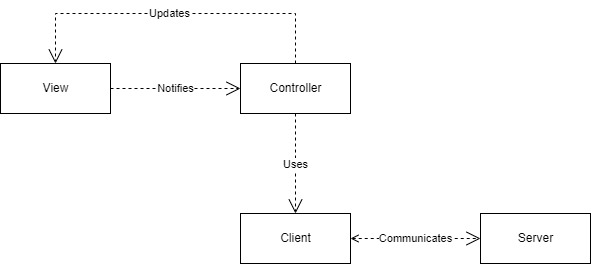
\includegraphics[width=\textwidth]{img/arch.jpg}
    \caption{Architettura MVC}
\end{figure}

\section{Design dettagliato}

\paragraph{GUI}
Nella versione con GUI, all'avvio dell'applicazione la pagina HTML viene connessa con la porta all'indirizzo 127.0.0.1:5000 e viene contemporaneamente lanciato il server come sotto-processo. Quest'ultimo viene anche aggiunto da codice alla lista dei sotto-processi che il processo padre (cioè l'applicazione stessa) deve "killare" quando termina; in questo modo la chiusura del server avviene in automatico, senza che l'utente debba interagire in alcun modo.

Per lo sviluppo del software è stato utilizzato Flask\footnote{\url{https://flask.palletsprojects.com/en/2.1.x/#}}, un micro-framework per Web Development, il quale permette, tra le altre cose, proprio di stabilire una connessione con una porta predefinita.

In questa versione dell'applicazione, l'utente interagisce con la pagina HTML (ascoltata e aggiornata dal sorgente javascript), che è collegata all'applicazione tramite il controller, rappresentato dallo script \textit{app.py}. In sostanza, la pressione di un pulsante da parte dell'utente scatena un interrupt software che viene gestito da un'opportuna funzione del controller, la quale inoltra la richiesta dell'utente alla specifica funzione del model in grado di gestirla. 
Il controller comunica solo con il client, il quale a sua volta interagisce con il server. 

Client e server sono stati scorporati in due file ciascuno, uno principale e uno di \textit{utility}, in un'ottica vicina al paradigma ad oggetti.

Alcune costanti particolarmente critiche per il corretto funzionamento dell'applicazione sono state dichiarate nel file \textit{settings.py}, utilizzato sia dal server che dal client. Tra queste costanti possiamo citare SERVER\_PORT, che stabilisce il numero della porta sulla quale verrà connesso il server e BUFFER\_SIZE, la quale serve a specificare la dimensione dei \textit{socket} utilizzati da client e server.

Ovviamente, qualora il server si trovasse su una macchina diversa dal client, il file condiviso settings.py dovrebbe essere copiato nella macchina dove viene eseguito il server.

Il design appena descritto è rappresentato nella figura in alto nella pagina seguente.
\begin{figure}[H]
    \centering
    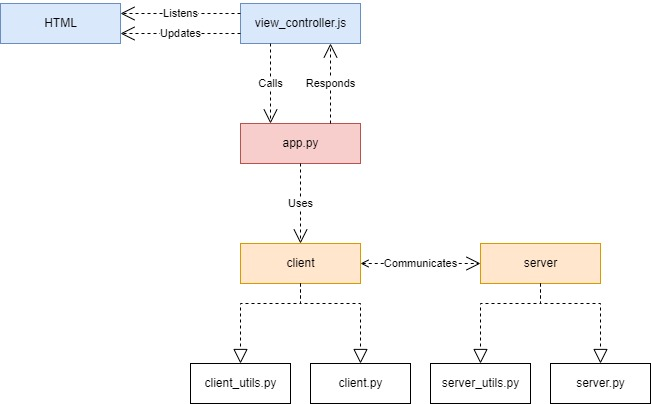
\includegraphics[width=\textwidth]{img/app_design.jpg}
    \caption{Design dell'applicazione utilizzata tramite GUI}
\end{figure}

\paragraph{Terminale} 
L'utilizzo dell'applicativo da terminale è supportato dal controller \textit{app\_cl.py}, progettato specificatamente per ricevere input da linea di comando. Tale controller invia al model il nome del comando digitato dall'utente ed eventualmente il file su cui operare.

Viene data all'utente la facoltà di chiudere la connessione con client e server tramite l'invio del comando \textit{quit}.

Per il resto valgono le stesse scelte di design descritte precedentemente, come si può vedere in figura:
\begin{figure}[H]
    \centering
    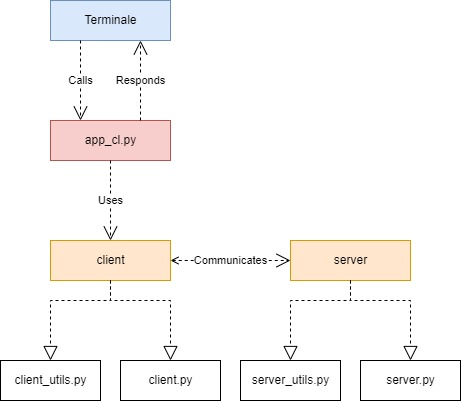
\includegraphics[scale=0.7]{img/cl_design.jpg}
    \caption{Design dell'applicazione utilizzata tramite terminale}
\end{figure}

\section{Descrizione delle operazioni}

\subsection{Gestione dei timeout}
Una problematica piuttosto complessa da gestire è stata l'implementazione del timeout, ossia il tempo massimo di attesa dell'arrivo di un segnale da parte del ricevente. 

Si è deciso di impostare il tempo ad un valore predefinito che dipende dal tipo di comunicazione in corso tra client e server.
In particolare, nel caso in cui il ricevente deve aspettare una messaggio testuale dal mittente il timeout è impostato a None (cioè 0 secondi), mentre nel caso in cui il ricevente deve aspettare l'arrivo dei pacchetti contenenti i dati del file da trasferire il timeout è imposto a 2 secondi.

Ciò significa che se l'arrivo di un messaggio testuale di acknowledgment viene ritardato oltre il valore del timeout, allora il mittente dovrà rispedire tale messaggio poiché il precedente viene considerato perso. Questa scelta garantisce una maggiore sicurezza nella comunicazione, anche se si pone in contrasto con i principi del protocollo UDP. 

Al contrario, l'arrivo dei pacchetti non è soggetto a timeout, quindi se un pacchetto viene perso il ricevente rimane bloccato ad aspettarlo, entrando in deadlock. Sebbene questa situazione sia tutt'altro che ideale, si è deciso per semplicità di supporre che tutti i pacchetti arrivino correttamente a destinazione.

\subsection{List}
Sotto l'aspetto implementativo l'operazione list è di gran lunga la più semplice. Il client invia il comando al server e aspetta di ricevere la lista di file in formato testuale. Il server, tramite la funzione di libreria \textit{os.listdir(path)} ottiene una lista di file e, dopo aver convertito la lista in stringa, invia il risultato al client.

In contrasto con quanto affermato nella sezione precedente, non è presente alcun timeout sull'arrivo della lista di file, nonostante il messaggio sia a tutti gli effetti di tipo testuale.

\begin{figure}[H]
    \centering
    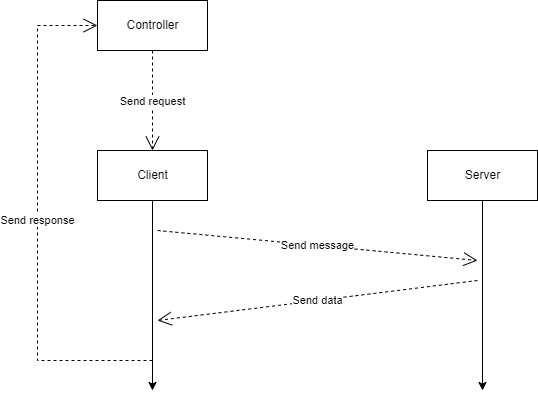
\includegraphics[scale=0.55]{img/list.jpg}
    \caption{Diagramma di sequenza dell'operazione list}
\end{figure}

\subsection{Get}
Prima di iniziare l'operazione vera e propria di download di un file dal server è necessario verificare che tale file sia presente nel server attraverso un controllo sul nome. Se il client possiede già un file con nome uguale a quello richiesto, il file viene comunque scaricato dal server e il file omonimo posseduto dal client viene sovrascritto, anche nel caso in cui il contenuto dei due file fosse identico.

Il server una volta ottenuto il nome del file richiesto dal client verifica se possiede un file con quel nome. In caso affermativo ritorna un messaggio di 'ACK' (acknowledgment) al client e poi spedisce il file desiderato, mentre in caso contrario manda un messaggio di 'NACK' (not acknowledgment). Se il server non ha ricevuto il nome del file perché è andato in timeout, allora lo chiede nuovamente al client tramite il messaggio 'RETRY'. \MakeUppercase{è} stato fissato un numero massimo di tentativi che il server ha per ottenere il nome del file, terminati i quali l'operazione viene dichiarata conclusa con esito negativo.

\begin{figure}[H]
    \centering
    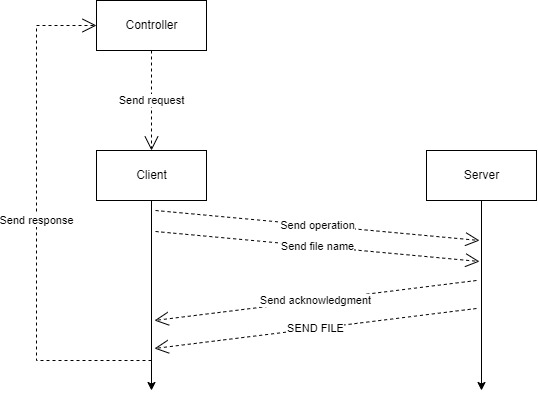
\includegraphics[scale=0.55]{img/get.jpg}
    \caption{Diagramma di sequenza dell'operazione get nel caso in cui la ricezione del nome del file da parte del server vada subito a buon fine}
\end{figure}

\subsection{Put}
L'operazione di put è piuttosto simile nel suo procedimento all'operazione di get appena descritta. Ovviamente, in questo caso è il client che deve verificare di possedere il file di cui fare l'upload.

Una differenza rispetto alla get è che quando il server ottiene il nome del file, esso re-invia il nome al client, che ne verifica la validità. In altre parole, il client controlla che il nome ottenuto dal server sia effettivamente quello che aveva spedito, così da evitare errori nel nome del file creato sul server. Se quest'ultimo possiede già un file omonimo del file di cui il client vuole fare l'upload, allora tale file viene eliminato.

Dopo questi controlli preliminari, il client spedisce il file al server.

\begin{figure}[H]
    \centering
    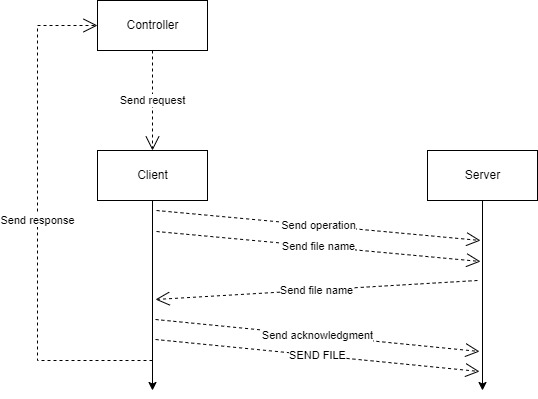
\includegraphics[scale=0.55]{img/put.jpg}
    \caption{Diagramma di sequenza dell'operazione put nel caso in cui il nome ottenuto dal server sia lo uguale a quello inviato dal client}
\end{figure}

\subsection{Trasferimento di un file}
L'operazione di trasferimento di un file è stata ovviamente quella più delicata ai fini della buona riuscita dell'applicazione.
Inizialmente viene creata una lista di pacchetti che il mittente deve spedire, ognuno formato da questi campi: 
\begin{itemize}
    \item \textit{content}, che contiene i dati letti dal file;
    \item \textit{pos}, che contiene la posizione del pacchetto nella lista di pacchetti;
    \item \textit{checksum}, che contiene una chiave hash che identifica univocamente il pacchetto stesso.
\end{itemize}
Successivamente viene spedito il numero di pacchetti al destinatario e infine, quando quest'ultimo conferma la ricezione del numero di pacchetti, il mittente invia il file un pacchetto alla volta.

Dal canto suo, il destinatario deve verificare che ogni pacchetto che arriva sia integro (verificando la validità del campo checksum) e poi quando tutti i pacchetti sono arrivati deve controllare che non ne sia andato perso nessuno. In base a queste verifiche il destinatario può accettare il contenuto ricevuto e quindi scriverlo sul nuovo file, oppure richiedere che gli venga inviato di nuovo (anche qui c'è un limite al numero di tentativi).

\begin{figure}[H]
    \centering
    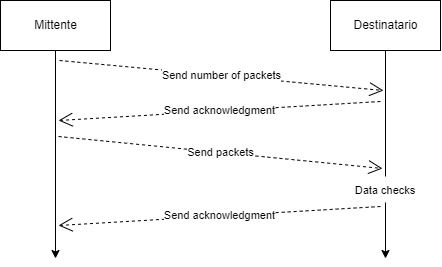
\includegraphics[scale=0.55]{img/transfer.jpg}
    \caption{Diagramma di sequenza del trasferimento di un file}
\end{figure}

\chapter{Sviluppo}

\section{Metodo di lavoro}
Dopo aver deciso di comune accordo il design di base e le librerie da utilizzare nello sviluppo del codice, i membri del gruppo si sono divisi i compiti e hanno lavorato ad una specifica componente del software. In particolare:
\begin{itemize}
    \item \textbf{Pasini} e \textbf{Sirri} hanno sviluppato client e server, con Pasini che si è occupato prevalentemente del client e Sirri del server. C'è stata comunque un'interazione continua, che ha permesso di uniformare le scelte implementative e di risolvere i problemi più difficili.  
    \item \textbf{Zavatta} si è occupato della parte di view, implementando il file HTML che definisce gli elementi grafici e lo script javascript che ne esegue l'aggiornamento quando l'utente compie una operazione. Inoltre, ha anche supportato lo sviluppo del model, fattorizzando opportunamente le operazioni del client in modo tale da renderle disponibili alla view.
\end{itemize}

Una decisione di gruppo importante è stata quella di dotare l'utente di due distinti metodi d'interazione con l'applicazione. Questa scelta è maturata dall'aver sviluppato in maniera quasi del tutto indipendente la parte di modello e quella di view.
La gestione del trasferimento di file tra client e server è stata infatti pensata (e testata) per input provenienti dalla riga di comando e quando si è andati a collegare la view a questa parte di model si è scelto di mantenere la possibilità di usare i comandi testuali.

\paragraph{Utilizzo di DVCS}
Per semplificare il lavoro in team si è fatto uso di Git come DVCS. Il workflow è stato quasi totalmente lineare, in quanto tutti i membri hanno sviluppato la propria parte di software sul branch master.

\chapter{Guida utente}
In entrambi i metodi di esecuzione è necessario avere una connessione a Internet attiva, poiché i fogli di stile (.css) vengono scaricati dalla Rete tramite Bootstrap all'avvio dell'applicazione.

\section{Terminale}
Dalla directory di progetto, lanciare da terminale Bash il comando '\textit{pyhton server.py}'. Successivamente, eseguire da un altro terminale l'applicazione tramite l'invio del comando '\textit{python app\_cl.py}'.

Il procedimento è andato a buon fine se nel terminale in cui è stata lanciata l'applicazione compare questo messaggio:
\begin{figure}[H]
    \centering
    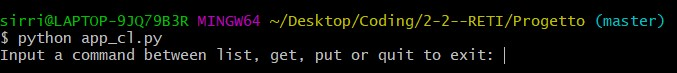
\includegraphics[width=\textwidth]{img/terminale.jpg}
\end{figure}

Dopo aver digitato il comando, è necessario attendere che ricompaia il messaggio di richiesta di input, in quanto questo è il segnale che l'applicazione ha terminato di gestire la richiesta precedente.
\begin{figure}[H]
    \centering
    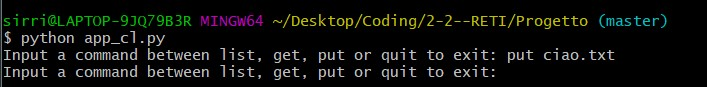
\includegraphics[width=\textwidth]{img/terminale_1.jpg}
\end{figure}

Per terminare l'applicazione digitare il comando \textit{quit} nella command line e premere invio. Questa operazione provoca anche la chiusura del server:
\begin{figure}[H]
    \centering
    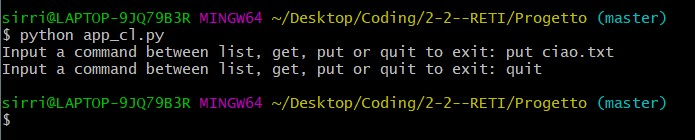
\includegraphics[width=\textwidth]{img/terminale_2.jpg}
\end{figure}

\section{Pagina HTML}
Lanciare il comando '\textit{python app.py}' in un terminale aperto nella directory di progetto. L'esecuzione di questo comando avvia automaticamente il server e produce l'output sottostante:
\begin{figure}[H]
    \centering
    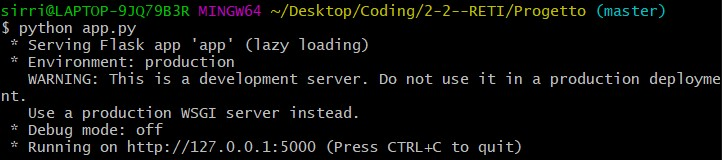
\includegraphics[width=\textwidth]{img/gui.jpg}
\end{figure}

Copiare l'indirizzo che si trova nell'ultima riga dell'output nella barra di ricerca di un qualsiasi browser e premere invio. Se tutto ha funzionato correttamente compare ora l'interfaccia grafica con cui poter interagire. I file presenti al momento sul server si trovano nella barra in basso:
\begin{figure}[H]
    \centering
    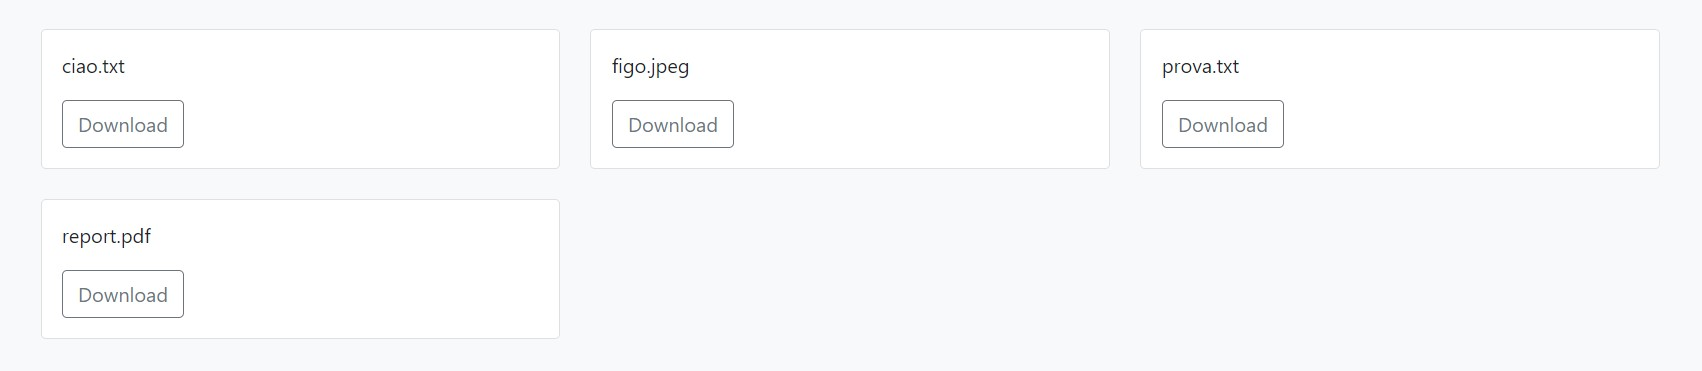
\includegraphics[width=\textwidth]{img/gui_1.jpg}
\end{figure}

I file posseduti dal client si ottengono cliccando sulla freccia a fianco del pulsante "Add file".
\begin{figure}[H]
    \centering
    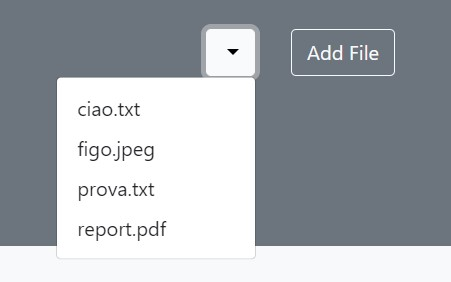
\includegraphics[scale=0.8]{img/gui_2.jpg}
\end{figure}

Per terminare definitivamente l'applicazione non è sufficiente chiudere la pagina HTML dal browser, poiché si deve prima terminare il processo da riga di comando.

\end{document}
